\documentclass[conference]{IEEEtran}
\IEEEoverridecommandlockouts
% The preceding line is only needed to identify funding in the first footnote. If that is unneeded, please comment it out.
\usepackage[noadjust]{cite}
\usepackage{amsmath,amssymb,amsfonts}
\usepackage{algorithmic}
\usepackage{graphicx}
\usepackage{textcomp}
\usepackage{xcolor}

\def\BibTeX{{\rm B\kern-.05em{\sc i\kern-.025em b}\kern-.08em
    T\kern-.1667em\lower.7ex\hbox{E}\kern-.125emX}}
\begin{document}

\title{Peningkatan Kinerja Modul Pencocokan Pola dalam Sistem Deteksi Intrusi Snort Menggunakan GPU\\
{\footnotesize \textsuperscript{*}Note: Sub-titles are not captured in Xplore and
should not be used}
\thanks{Identify applicable funding agency here. If none, delete this.}
}

\author{
\IEEEauthorblockN{Afrizal Fikri}
\IEEEauthorblockA{{School of Electrical Engineering and Informatics} \\
{Institut Teknologi Bandung}\\
{Bandung, Indonesia} \\
afrizalf96@gmail.com}
\and
\IEEEauthorblockN{Achmad Imam Kistijantoro}
\IEEEauthorblockA{{School of Electrical Engineering and Informatics} \\
{Institut Teknologi Bandung}\\
{Bandung, Indonesia} \\
imam@informatika.org}
}

\maketitle

\begin{abstract}
    The advancement of technology has been giving contributions to the rapid growth of the use of digital data. In this digital era, lots of physical data have been transformed into the digital ones. Among those, a lot of confidential data also take place. Thus, security assurance become important as well. One of the entry point of those malicious usages come from server side. Ensuring authority on server utilizing network intrusion detection system (NIDS) could take enormous resource and time. One of the important part of NIDS is string matching part inside the analyzer. Based on this rationale, this paper aims to improve matching speed of detection in order to maximize overall system throughput using GPU instead of CPU. Based on the experiment and testing, the proposed solution has a significantly better run time compared to the state of the art linear solution while maintaining the accuracy. 
\end{abstract}

\begin{IEEEkeywords}
    pattern matching; intrusion detection; GPU; parallel computation; CUDA
\end{IEEEkeywords}

\section{Introduction}
The advancement of technology has given contributions to the rapid growth of the use of digital data. In this digital era, lots of physical data have been transformed into the digital ones. One example of the use of digital data is the digital biometric fingerprint data on the Electronic Identity Card (KTP-el). 

To identify a person, fingerprint matching can be used. There are some techniques to do fingerprint matching. One of popular technique is minutia-based fingerprint matching [1]. The technique can be classified into two categories, nearest neighbor-based and fixed radius-based. Each category has their own advantages and disadvantages. However, there is a technique that combines their advantages without having their drawbacks, i.e. Minutia Cylinder-Code (MCC). 

Fingerprint matching is a problem, especially in a country that has a large population. According to Indonesian 2010 census, it was found that the total population of Indonesia was approximately 237.641.326 at that time [2]. In regard to this matter, the process of analyzing their fingerprints data could take extremely long time if it done linearly, which is what is currently happening. Thus, there is a need for a parallel fingerprint matching.

Parallel processing can be done with multicore CPU, multicore GPU, or multicomputer. The difference between CPU and GPU is how they process task [3]. CPU only has several cores designed to process sequentially, while GPU has thousands of cores designed to do tasks in parallel.

Based on previous statements, this paper aims to optimize fingerprint matching using Minutia Cylinder-Code with GPU. The optimization will be evaluated and the performance will be compared to the baseline.

\section{String Matching}
In general, there are two kinds of string matching: single pattern string matching and multi pattern string matching. We will focus into multi pattern string matching. There are several famous algorithms for multi pattern string matching: Aho-Corasick, Commentz-Walter, and Wu-Manber algorithm. This paper will try to implement variation of Aho-Corasick algorithm.

    \subsection{Aho-Corasick Algorithm}
    Aho-Corasick algorithm is kind of string matching algorithm works by matching one string to a dictionary. This dictionary contains all pattern to be matched in form state machine. 
    
    In this algorithm, matching operation is performed by traversing state machine by characters in input string. If any of the final state reached, then input string matched one of the patterns. Matching continued until input string is terminated. 

    \begin{figure}[htbp]
        \centerline{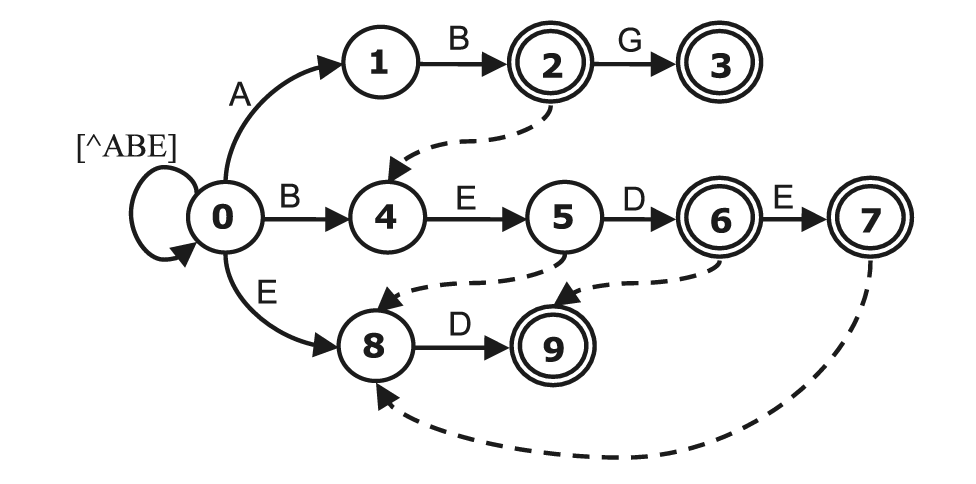
\includegraphics[width=0.4\textwidth]{../src/resources/aho-c.png}}
        \caption{Example state machine of Aho-Corasick dictionary.}
    \end{figure}

    Aho-Corasick use failure function to perform backtrack after stop at one of the final states. Failure function will redirect this final state to longest pattern prefix which match suffix of the currently matched pattern. Failure function reduce the need of repeating another same sequence which just matched by. By this method, all of containing patterns can be matched by one pass and reducing complexity from $O(mn)$ to $O(n)$. 

    In this algorithm, memory lookup become bottleneck. Every traversal operation will fetch one entry from table. Since memory accesses are more expensive than computations, this algorithm is memory bound.

    \subsection{Data Parallel Aho-Corasick}
    In order to extend Aho-Corasick into multithreading, we need to divide the load of matching for each threads. One of the method is by partitioning input into several chunks and then each threads will match this sequence into dictionary. But as we encounter a pattern span multiple chunks at once, it is not recognized on either threads. This problem known as boundary detection problem. So, we need to extend matching by length of the longest pattern. Memory lookup thus increase to $O((n/s + m) * s) = O(n + ms)$ for $s$ is amount of chunks. 

    \begin{figure}[htbp]
        \centerline{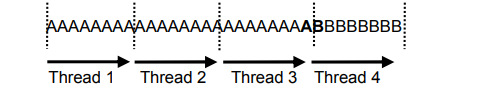
\includegraphics[width=0.4\textwidth]{../src/resources/boundary.png}}
        \caption{Pattern \textbf{AB} not recognized by both thread 3 and 4}
    \end{figure}

    \subsection{Parallel Failureless Aho-Corasick}
    Another method to adapt multithreading Aho-Corasick is to spread threads to all characters byte. Each threads will matching any pattern begin with each coresponding character and terminate if any of final state or no valid transition occurs \cite{lin2013}. The consequence is eavery character will match only one pattern at most.
    Thus, no need to make any failure function. And also boundary detection problem will not occur by using this approach. This approach named as Parallel Failureless Aho-Corasick (PFAC).

    \begin{figure}[htbp]
        \centerline{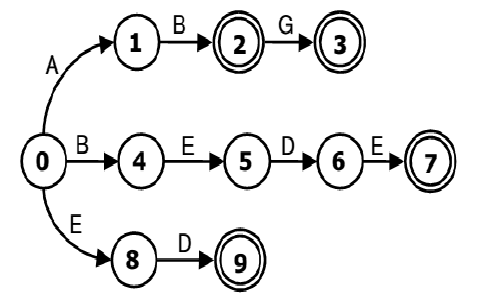
\includegraphics[width=0.4\textwidth]{../src/resources/pfac.png}}
        \caption{State machine without failure function}
    \end{figure} 

\section{Related Works}

    \subsection{Utilization of Double Buffering Scheme, Texture Memory and Pinned Memory}

        In this paper, GPU-based matching implementation had been proposed using Aho-Corasick algorithm. Beside utilization of GPU multithreading, there are few adjustment to import Aho-Corasick to GPGPU. State machine built using transition table on 2D table on texture memory. Based on experiment, this implementation improving performance by 19\% \cite{gnort2008}.
        
        For the memory transfer scheme, double buffering scheme was proposed. Packets will be batched in one buffer. Whenever the buffer gets full, all packets are transferred to the GPU in one operation. Transfer from device to host also done in same way. All result will be batched in the second buffer and get transferred when gets full.
        
        Another optimization trick used is using pinned memory. Both of the buffer in host will be pinned to reduce swappiness. And pinned memory also enable DMA transfer and reducing computation needs and latency. This design could improve system performance until 3.2 times higher than implementation using multithreading on CPU.

    \subsection{Scalable Architecture for Maximizing GPU Utilization}

        By profiling, it is concluded that bottleneck occured on 3 components: packet acquisition, multi pattern string matching, and option rule matching by regular expression. Moreover, inside string matching component alone, average utilization of GPU still low. This paper applied architectural improvement around NIDS. \textcolor{red}{Methods being proposed} are pipelining and payload batching. Pipelining used to separate thread using in transfer and matching. And by this architecture, NIDS can be scaled to multiple GPU and CPU core instances \cite{kargus2012}. 
        
        Improvement achieved by this method was about 1.5 until 4 times higher compared to Snort baseline. Evaluation performed using double CPU Intel X5680 with 12 core each and double GPU NVIDIA GTX 580. NIDS was run under network traffic with capacity around 40 Gbps and could reach throughput 25.2 Gbps.

    \subsection{Failureless Aho-Corasick by Maximizing Shared Memory Usage}

        One way to perform Aho-Corasick matching is by assigning each input byte to each threads simultanously. Then each threads will perform matching \textcolor{red}{begin} with assined byte. Matching stops whenever final state or invalid transition occurs. This approach need no failure function. So that each thread only responsible for matching at most one pattern \cite{lin2013}.
        
        This novel approach utilizing memory coalescing in GPU so sequential bytes can be loaded at once. To further improve performance, transition from beginning state will be loaded to shared memory to reduce transaction toward global memory. 
        
        For the transition table, we cannot ensure it will fit to the shared memory. So in alternative to shared memory, transition table will be bound to texture memory instead. Texture memory has several advantages. Texture memory has bigger cache and suitable to perform fetching with access pattern which are difficult to predict. Testing using PCAP dataset from DEFCON showed significant performance improvement. Using CPU Intel Core i7-950 and GPU NVIDIA GTX 580, system throughput could become 3 times compared to Snort baseline.

\section{Proposed Solution}
    \subsection{Matching Algorithm}
        In order to implement Aho-Corasick to GPU, we need to exploit SIMD (single instruction multiple data) optimally. Data parallel approach is one of the easiest approach to implement. After splitting chunks, each chunks assign to different threads with extension as long the longest pattern. This approach has 2 problem: the extension increasing data transaction drastically, and not optimal if input splitted to so many chunks. \textcolor{red}{GPU can spawn as hundreds threads and hopefully all threads can be utilized optimally.}

        Alternative solution is by using PFAC. The idea of allocating an individual thread to each byte of an input stream has important implications on the efficiency of the PFAC state machine. 
        
        % First, each thread of PFAC is only responsible for identifying the pattern starting at the thread’s starting position. Therefore, whenever a thread cannot find any pattern located at its beginning position, it terminates immediately without taking failure transitions to backtrack the state machine. In other words, each thread of PFAC runs in the best time $O(1)$ and the worst time $O(m)$ where $m$ is the longest pattern length. Therefore, the failure transitions of the AC state machine are all removed as well as the self-loop transition of the initial state. An AC state machine with all its failure transitions and self-loop transition removed is called a PFAC machine. Fig. 4 shows the PFAC machine to identify the four patterns, “AB,” “ABG,” “BEDE,” and “ED.”

        \begin{enumerate}
            \item Each thread only be responsible to sequence begins with a character. If there is no match pattern, thread will terminate immediately. Consequently, threads will only last for a short period.

            \item Matching done parallel in warp of 32 threads. Thus, the memory access of those will be coalesced and improve the throughput.

            \item Have no additional space for failure transition. Memory consumption become more efficient and cache hit chances become bigger.
        \end{enumerate}

        % Huntul ngaceng

    \subsection{State Machine Implementation}
        There are 2 alternatives for state machine implementation: two-dimensional table or trie with pointer. Structure of trie support dynamic modification and link-unlinking. But it is too complex to be stored in GPU. And also memory place could become fragmented and cannot exploit spatial locality. Not to mention the cost allocating memory in GPU is too demandly. So, this option is less preferable. 

        Another design and the easier is two-dimensional table. For each states, there will be transition to, say 256 characters (if the input is unsigned ASCII char). This model is simple and support memory coalescing. If we utilize texture memory, also there will be chances access pattern will be cached.

        After all pattern registered, table will be compiled in the host. And then, table get transferred to device just as the size of filled table. ``Fig.~\ref{table}'' below shows the design of transition table.

    \begin{figure}[htbp]
        \centerline{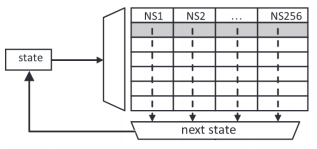
\includegraphics[width=0.4\textwidth]{../src/resources/table.png}}
        \caption{Transition table representation}
        \label{table}
    \end{figure}

    \subsection{Thread Allocation}
        Problem for using PFAC is load of each threads can be unbalanced (because of only few threads will survived)
        Solution: repeating assignment

    \subsection{GPU Optimation}
        Load input to shared
        Load first row to shared
        Bind to texture
        Bind to pinned
        Thread reduce bank conflict

\section{Implementation on Snort}
    \subsection{MPSE Interface}
        What provided? And how you implement those interface?

    \subsection{Modules}
        Connect interface to your design

\section{Evaluation}
    \subsection{Environment}
        asd
        
    \subsection{Performance Evaluation}
        asd

\section{Conclusion}

    % \begin{table}[htbp]
    % \caption{Table Type Styles}
    % \begin{center}
    % \begin{tabular}{|c|c|c|c|}
    % \hline
    % \textbf{Table}&\multicolumn{3}{|c|}{\textbf{Table Column Head}} \\
    % \cline{2-4} 
    % \textbf{Head} & \textbf{\textit{Table column subhead}}& \textbf{\textit{Subhead}}& \textbf{\textit{Subhead}} \\
    % \hline
    % copy& More table copy$^{\mathrm{a}}$& &  \\
    % \hline
    % \multicolumn{4}{l}{$^{\mathrm{a}}$Sample of a Table footnote.}
    % \end{tabular}
    % \label{tab1}
    % \end{center}
    % \end{table}

    % \begin{figure}[htbp]
    % \centerline{\includegraphics{fig1.png}}
    % \caption{Example of a figure caption.}

    % \end{figure}

\section{Acknowledgment}

\bibliography{references}
\bibliographystyle{IEEEtran}

\end{document}
